\documentclass[12pt]{article}

% PACKAGES
\usepackage{amsmath} % For advanced math environments
\usepackage{geometry} % For setting page margins
\usepackage{graphicx} % For including images
\usepackage{tikz} % For drawing diagrams
\usepackage{amsfonts} % For math fonts
\usepackage{amssymb} % For more math symbols
\usepackage{fancyhdr} % For headers and footers
\usepackage{tcolorbox} % For colored boxes around problems
\usepackage{siunitx} % For SI units

% DOCUMENT SETUP
\geometry{a4paper, margin=1in}
\pagestyle{fancy}
\fancyhf{}
\rhead{Microscopes \& Telescopes}
\lhead{Teaching Notes \& Problems}
\cfoot{\thepage}

\title{\textbf{Teaching Notes: Microscopes \& Telescopes}}
\author{Gemini}
\date{\today}

\begin{document}

\maketitle
\thispagestyle{empty}
\tableofcontents
\newpage

\section{The Compound Microscope \(\text{\normalsize \reflectbox{}}\)}

A \textbf{compound microscope} is used to view very small objects that are placed close to it. It uses two converging lenses to produce a highly magnified virtual image.
\begin{figure}[h!]
\centering
% This code is designed to faithfully replicate the user-provided image.
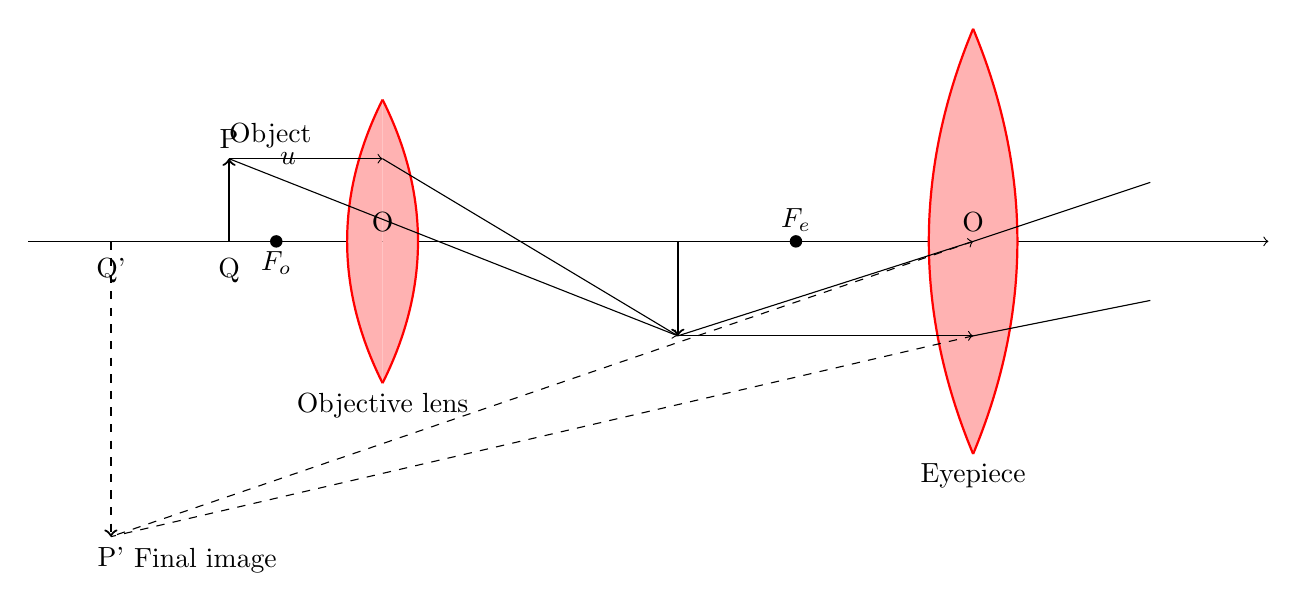
\begin{tikzpicture}[scale=1.5]

    % Principal Axis
    \draw (0,0) -- (10,0); % Line without arrow at start
    \draw[->] (10,0) -- (10.5,0); % Arrow at the end of the principal axis

    % Q' and Q labels
    \node at (0.7, -0.25) {Q'};
    \node at (1.7, -0.25) {Q};

    % Objective Lens
    \begin{scope}[shift={(3,0)}, scale=0.8]
        \draw[thick, red, fill=red!30] (0,1.5) .. controls (0.5,0.5) and (0.5,-0.5) .. (0,-1.5);
        \draw[thick, red, fill=red!30] (0,1.5) .. controls (-0.5,0.5) and (-0.5,-0.5) .. (0,-1.5);
        \node[below, black] at (0,-1.5) {Objective lens};
        \node[above, black] at (0,0) {O}; % Optical center of objective
    \end{scope}

    % Eyepiece
    \begin{scope}[shift={(8,0)}, scale=1.0]
        \draw[thick, red, fill=red!30] (0,1.8) .. controls (0.5,0.6) and (0.5,-0.6) .. (0,-1.8);
        \draw[thick, red, fill=red!30] (0,1.8) .. controls (-0.5,0.6) and (-0.5,-0.6) .. (0,-1.8);
        \node[below, black] at (0,-1.8) {Eyepiece};
        \node[above, black] at (0,0) {O}; % Optical center of eyepiece
    \end{scope}

    % Object P
    \draw[thick, ->] (1.7,0) -- (1.7,0.7) node[above] {P};
    \node at (2.05, 0.9) {Object};
    \node at (2.2, 0.7) {$u$}; % Label u

    % Focal Points as shown in the image
    \fill (2.1,0) circle (1.5pt) node[below] {$F_o$}; % Objective's focal point
    \fill (6.5,0) circle (1.5pt) node[above] {$F_e$}; % Eyepiece's focal point (primary)

    % --- Rays from Object to form the Intermediate Image ---
    % Ray 1: Parallel to axis, then through objective's focal point
    \draw[->] (1.7,0.7) -- (3,0.7); % To objective lens
    \draw (3,0.7) -- (5.5, -0.8);    % From objective lens, converges
    % Ray 2: Through optical center of objective, undeviated
    \draw[->] (1.7,0.7) -- (5.5, -0.8); % Through O of objective

    % --- Intermediate Image ---
    \draw[thick, ->] (5.5,0) -- (5.5,-0.8); % Formed by objective

    % --- Rays from Intermediate Image through Eyepiece ---
    % Ray 1: From intermediate image, through center of eyepiece, undeviated
    \draw[->] (5.5,-0.8) -- (8,0); % To eyepiece center
    \draw (8,0) -- (9.5, 0.5);      % Emerging ray 1
    % Ray 2: From intermediate image, parallel to axis, then refracts
    \draw[->] (5.5,-0.8) -- (8, -0.8); % To eyepiece, parallel to axis
    \draw (8, -0.8) -- (9.5, -0.5); % Emerging ray 2

    % --- Dashed lines to form the Final Image (traced backwards) ---
    % These dashed lines are extensions of the emerging rays, meeting at P'
    \draw[dashed] (8,0) -- (0.7, -2.5);   % Extension of emerging ray 1
    \draw[dashed] (8,-0.8) -- (0.7, -2.5); % Extension of emerging ray 2

    % --- Final Image P'Q' ---
    \draw[thick, ->, dashed] (0.7,0) -- (0.7,-2.5) node[below] {P'};
    \node at (1.5, -2.7) {Final image};

\end{tikzpicture}
\caption{Ray diagram for a compound microscope, replicating the provided image.}
\end{figure}

\subsection{Key Components \& Setup}
\begin{enumerate}
    \item \textbf{Objective Lens:} This is the lens closer to the object. It has a \textbf{very short focal length} ($f_o$).
    \item \textbf{Eyepiece (Ocular):} This is the lens you look through. It has a \textbf{longer focal length} ($f_e$) than the objective.
\end{enumerate}

The objective lens creates a \textbf{real, inverted, and magnified} intermediate image. The eyepiece then acts like a simple magnifying glass to view this intermediate image, creating a \textbf{final, virtual, and even more magnified} image.


\subsection{Essential Equations}
\begin{itemize}
    \item \textbf{Thin Lens Formula} (applies to both lenses):
    $$ \frac{1}{f} = \frac{1}{u} + \frac{1}{v} $$
    where $f$ is focal length, $u$ is object distance, and $v$ is image distance. Sign Convention: Distances for real objects/images are positive; for virtual images, $v$ is negative. $f$ is positive for converging lenses.
    
    \item \textbf{Lens Separation ($L$):} The distance between the objective and the eyepiece.
    $$ L = v_o + u_e $$
    where $v_o$ is the image distance for the objective and $u_e$ is the object distance for the eyepiece.
    
    \item \textbf{Magnifying Power ($M$):} The total angular magnification.
    $$ M = m_o \times M_e $$
    where $m_o$ is the linear magnification of the objective ($m_o = \frac{v_o}{u_o}$) and $M_e$ is the angular magnification of the eyepiece ($M_e = \frac{D}{u_e}$). $D$ is the near point of the eye, typically taken as \SI{250}{\milli\meter}.
\end{itemize}

\newpage

\section{The Astronomical Telescope \(\text{\normalsize }\)}
An \textbf{astronomical telescope} is used to view very large objects that are extremely far away. It also uses two converging lenses.

\subsection{Key Components \& Setup}
\begin{enumerate}
    \item \textbf{Objective Lens:} Closer to the distant object. It has a \textbf{long focal length} ($f_o$).
    \item \textbf{Eyepiece (Ocular):} The lens you look through. It has a \textbf{short focal length} ($f_e$).
\end{enumerate}
Since the object is at infinity, the objective lens forms a real, inverted image at its focal point ($f_o$). The eyepiece then magnifies this image.

\subsection{Normal Adjustment}
This is the standard configuration where the \textbf{final image is formed at infinity}. This occurs when the intermediate image (formed at $f_o$) is placed exactly at the focal point of the eyepiece ($f_e$).

\subsection{Ray Diagram (Normal Adjustment)}
\begin{figure}[h!]
\centering
% This code is designed to faithfully replicate the user-provided telescope diagram,
% with special attention to ensuring rays are correctly drawn in parallel.
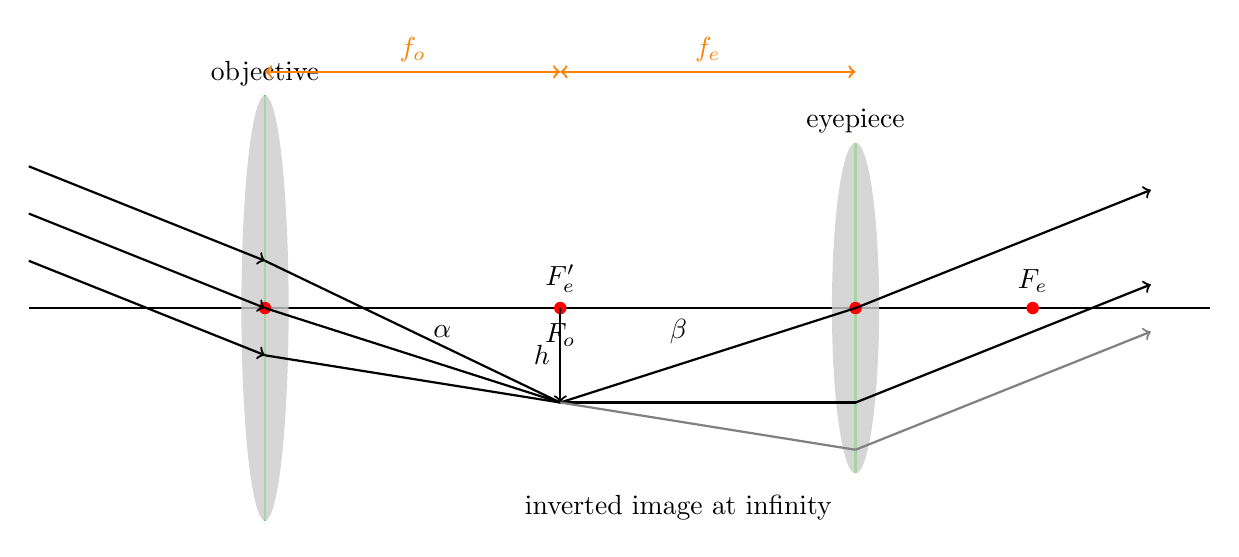
\begin{tikzpicture}[scale=1.5]

    % --- Principal Axis ---
    \draw (0,0) -- (10,0);

    % --- Lenses ---
    % Objective Lens
    \draw[green, thick] (2, -1.8) -- (2, 1.8);
    \fill[gray!40, opacity=0.8] (2,0) ellipse (0.2cm and 1.8cm);
    \node[above] at (2,1.8) {objective};
    \fill[red] (2,0) circle (1.5pt);

    % Eyepiece Lens
    \draw[green, thick] (7, -1.4) -- (7, 1.4);
    \fill[gray!40, opacity=0.8] (7,0) ellipse (0.2cm and 1.4cm);
    \node[above] at (7,1.4) {eyepiece};
    \fill[red] (7,0) circle (1.5pt);

    % --- Focal Points and Labels ---
    \node[below] at (4.5,-0.05) {$F_o$};
    \fill[red] (4.5,0) circle (1.5pt);
    \node[above] at (4.5,0.05) {$F_e'$};
    \node[above] at (8.5,0.05) {$F_e$};
    \fill[red] (8.5,0) circle (1.5pt);

    % --- Focal Length markers ---
    \draw[<->, orange, thick] (2, 2) -- (4.5, 2) node[midway, above] {$f_o$};
    \draw[<->, orange, thick] (4.5, 2) -- (7, 2) node[midway, above] {$f_e$};

    % --- Rays from Objective ---
    % Incoming rays are PARALLEL to each other, entering at an angle.
    \draw[thick, ->] (0, 1.2) -- (2, 0.4); % Top ray
    \draw[thick, ->] (0, 0.4) -- (2, -0.4); % Bottom ray
    % The central ray defines the angle for all incoming parallel rays.
    \draw[thick, ->] (0, 0.8) -- (2, 0); % Ray heading for the optical center

    % Refracted rays converging at the focal point F_o
    \draw[thick] (2, 0.4) -- (4.5, -0.8);
    \draw[thick] (2, 0) -- (4.5, -0.8);
    \draw[thick] (2, -0.4) -- (4.5, -0.8);

    % --- Intermediate Image ---
    \draw[thick, ->] (4.5,0) -- (4.5,-0.8) node[midway, left] {$h$};

    % --- Rays from Eyepiece ---
    % These rays MUST emerge PARALLEL to each other.
    % Ray 1 (Central Ray): Passes through the center of the eyepiece undeviated.
    % This ray's direction determines the direction of all other emerging parallel rays.
    \draw[thick] (4.5, -0.8) -- (7, 0);
    \draw[thick, ->] (7, 0) -- (9.5, 1);

    % Ray 2: From intermediate image, parallel to axis, then through F_e.
    % This must emerge parallel to the central ray.
    \draw[thick] (4.5, -0.8) -- (7, -0.8);
    \draw[thick, ->] (7, -0.8) -- (9.5, 0.2); % Drawn parallel to the ray above

    % Ray 3 (Gray helper ray from diagram): From intermediate image.
    \draw[thick, gray] (4.5, -0.8) -- (7, -1.2);
    \draw[thick, ->, gray] (7, -1.2) -- (9.5, -0.2); % Drawn parallel to the other two

    % --- Angle indicators ---
    \node at (3.5, -0.2) {$\alpha$};
    \node at (5.5, -0.2) {$\beta$};

    % --- Final Image Label ---
    \node[below] at (5.5,-1.5) {inverted image at infinity};

\end{tikzpicture}
\caption{A ray diagram for an astronomical telescope with correctly drawn parallel incoming and emerging rays, as per your guide.}
\end{figure}


\subsection{Essential Equations (Normal Adjustment)}
\begin{itemize}
    \item \textbf{Lens Separation ($L$):}
    $$ L = f_o + f_e $$
    \item \textbf{Magnifying Power ($M$):}
    $$ M = \frac{f_o}{f_e} $$
\end{itemize}

\newpage
\section{Problem Solving}

\subsection{Problem 1: Compound Microscope (SPhO 2020)}
\begin{tcolorbox}[colback=blue!5!white,colframe=blue!75!black,title=Question]
A compound microscope contains two thin lenses of focal length \SI{6.0}{\milli\meter} and \SI{40.0}{\milli\meter}, respectively. The lenses are separated by a distance of \SI{200}{\milli\meter}. The final image is formed \SI{250}{\milli\meter} from the eye lens. Calculate
\begin{itemize}
    \item[(i)] The distance of the object from the objective lens.
    \item[(ii)] The magnifying power of the microscope.
\end{itemize}
\end{tcolorbox}

\subsubsection{Explanation and Solution}
\textbf{Given values:}
\begin{itemize}
    \item Objective focal length, $f_o = \SI{6.0}{\milli\meter}$.
    \item Eyepiece focal length, $f_e = \SI{40.0}{\milli\meter}$.
    \item Lens separation, $L = \SI{200}{\milli\meter}$.
    \item Final image distance from eyepiece, $v_e = \SI{-250}{\milli\meter}$ (negative for a virtual image).
    \item Near point, $D = \SI{250}{\milli\meter}$.
\end{itemize}

\begin{enumerate}
    \item \textbf{Analyze the Eyepiece:} Find the position of the intermediate image ($u_e$) using the lens formula for the eyepiece.
    $$ \frac{1}{f_e} = \frac{1}{u_e} + \frac{1}{v_e} $$
    $$ \frac{1}{40.0} = \frac{1}{u_e} + \frac{1}{-250} $$
    $$ \frac{1}{u_e} = \frac{1}{40.0} + \frac{1}{250} = \frac{25 + 4}{1000} = \frac{29}{1000} $$
    $$ u_e = \frac{1000}{29} \approx \SI{34.48}{\milli\meter} $$
    
    \item \textbf{Find the Objective's Image Distance ($v_o$):} Use the lens separation formula.
    $$ L = v_o + u_e $$
    $$ 200 = v_o + 34.48 \implies v_o = 200 - 34.48 = \SI{165.52}{\milli\meter} $$
    
    \item \textbf{Analyze the Objective Lens (Answer for part i):} Find the original object's distance ($u_o$) using the lens formula for the objective.
    $$ \frac{1}{f_o} = \frac{1}{u_o} + \frac{1}{v_o} $$
    $$ \frac{1}{6.0} = \frac{1}{u_o} + \frac{1}{165.52} $$
    $$ \frac{1}{u_o} = \frac{1}{6.0} - \frac{1}{165.52} = \frac{165.52 - 6.0}{6.0 \times 165.52} = \frac{159.52}{993.12} $$
    $$ u_o = \frac{993.12}{159.52} \approx \SI{6.226}{\milli\meter} $$
    \textbf{Answer (i): The object distance is approximately \SI{6.23}{\milli\meter}.}
    
    \item \textbf{Calculate Magnifying Power (Answer for part ii):}
    $$ M = m_o \times M_e = \left(\frac{v_o}{u_o}\right) \times \left(\frac{D}{u_e}\right) $$
    $$ M = \left(\frac{165.52}{6.226}\right) \times \left(\frac{250}{34.48}\right) $$
    $$ M \approx (26.59) \times (7.25) \approx 192.8 $$
    \textbf{Answer (ii): The magnifying power is approximately 193.}
\end{enumerate}

\newpage

\subsection{Problem 2: Astronomical Telescope (SPhO 2023)}
\begin{tcolorbox}[colback=red!5!white,colframe=red!75!black,title=Question]
The distance between the objective lens and the eyepiece of an astronomical telescope in its normal adjustment is \SI{105}{\centi\meter}. When the eyepiece is moved \SI{1.0}{\centi\meter} towards the objective lens, a final virtual image is formed at a point \SI{20}{\centi\meter} from the eyepiece. Calculate the focal lengths of the objective lens and of the eyepiece.
\end{tcolorbox}

\subsubsection{Explanation and Solution}
\textbf{Given values:}
\begin{itemize}
    \item \textbf{Case 1 (Normal Adjustment):}
    \begin{itemize}
        \item Lens separation, $L_1 = \SI{105}{\centi\meter}$.
        \item Final image is at infinity.
    \end{itemize}
    \item \textbf{Case 2 (Adjusted):}
    \begin{itemize}
        \item New separation, $L_2 = 105 - 1.0 = \SI{104}{\centi\meter}$.
        \item Final virtual image distance, $v_e = \SI{-20}{\centi\meter}$.
    \end{itemize}
\end{itemize}

\begin{enumerate}
    \item \textbf{Formulate Equation from Case 1:} In normal adjustment:
    $$ L_1 = f_o + f_e $$
    \begin{equation}
        105 = f_o + f_e \label{eq:A}
    \end{equation}
    
    \item \textbf{Formulate Equations from Case 2:} The intermediate image is still formed at $f_o$ from the objective. The new separation is:
    $$ L_2 = f_o + u_e $$
    \begin{equation}
        104 = f_o + u_e \label{eq:B}
    \end{equation}
    For the eyepiece in this new position, the lens formula is:
    \begin{equation}
        \frac{1}{f_e} = \frac{1}{u_e} + \frac{1}{v_e} = \frac{1}{u_e} - \frac{1}{20} \label{eq:C}
    \end{equation}
    
    \item \textbf{Solve the System of Equations:} We have three equations for $f_o, f_e, u_e$.
    \begin{itemize}
        \item From Eq. \eqref{eq:A}, express $f_o$: $f_o = 105 - f_e$.
        \item Substitute this into Eq. \eqref{eq:B}:
        $$ 104 = (105 - f_e) + u_e \implies u_e = f_e - 1 $$
        \item Substitute this expression for $u_e$ into Eq. \eqref{eq:C}:
        $$ \frac{1}{f_e} = \frac{1}{f_e - 1} - \frac{1}{20} $$
        \item Rearrange to solve for $f_e$:
        $$ \frac{1}{20} = \frac{1}{f_e - 1} - \frac{1}{f_e} = \frac{f_e - (f_e - 1)}{f_e(f_e - 1)} = \frac{1}{f_e(f_e - 1)} $$
        \item This leads to a quadratic equation:
        $$ f_e^2 - f_e = 20 \implies f_e^2 - f_e - 20 = 0 $$
        \item Factor the quadratic:
        $$ (f_e - 5)(f_e + 4) = 0 $$
    \end{itemize}
    The solutions are $f_e = 5$ or $f_e = -4$. Since the eyepiece of an astronomical telescope is a converging lens, its focal length must be positive.
    $$ \mathbf{f_e = \SI{5.0}{\centi\meter}} $$
    
    \item \textbf{Find the Objective Focal Length ($f_o$):} Substitute $f_e$ back into Eq. \eqref{eq:A}:
    $$ f_o = 105 - f_e = 105 - 5 = \SI{100}{\centi\meter} $$
    
    \textbf{Final Answer: The focal length of the objective is \SI{100}{\centi\meter} and the focal length of the eyepiece is \SI{5.0}{\centi\meter}.}
\end{enumerate}

\end{document}